\documentclass[12pt, letterpaper]{article}

% Packages for formatting
\usepackage[margin=1in]{geometry}
\usepackage{mathptmx} % Times New Roman font
\usepackage{setspace}
\singlespacing 
\usepackage{enumitem}
\usepackage{hyperref}
\usepackage{titlesec}
\usepackage{cite} % For handling citations
\usepackage{graphicx}
\usepackage{float}

% Section formatting
\titleformat{\section}{\large\bfseries}{}{0em}{}
\titlespacing{\section}{0pt}{1.5ex plus 1ex minus .2ex}{1ex plus .2ex}

\begin{document}

\begin{center}
    \textbf{\Large Midterm Report: Evaluating Small Fact-Checkers in Natural Long-Context Scenarios} \\
    \vspace{0.5em}
    \textbf{Chenan Wang} \\
    \textbf{Project Type:} Research / Implementation
\end{center}

\vspace{1em}

\section*{B. Introduction}

Current lightweight fact-checking models, such as MiniCheck \cite{tang2024minicheck}, are predominantly trained and evaluated on short, paragraph-level snippets (typically chunked to 350-500 tokens). However, in realistic Retrieval-Augmented Generation (RAG) pipelines, the context is often much longer and heavily populated with irrelevant or conflicting information. 

Our primary motivation is to understand how these lightweight fact-checkers (<1B parameters, such as MiniCheck-FT5, and larger variants like Bespoke-MiniCheck-7B) behave when exposed to naturally long-context datasets spanning from 500 to over 74,000 tokens. As LLM context windows grow, running fact-checking over massive retrieved documents becomes computationally expensive. It is currently an open question whether the local chunking mechanisms employed by models like MiniCheck \cite{tang2024minicheck} and AlignScore \cite{zha2023alignscore} can survive similar long-context stress tests without suffering significant accuracy degradation.

\section*{C. Related Work}

Current standardized factuality methods such as AlignScore \cite{zha2023alignscore} and MiniCheck \cite{tang2024minicheck} rely on fixed-length, relatively clean grounding documents. MiniCheck itself is an optimal setup that chunks long documents into around 400-word pieces, retrieving maximum support probabilities. However, recent studies indicate that LLMs frequently fail to utilize information buried in the middle of extended contexts \cite{laban2024summary}. Our work bridges these two domains: we apply the rigorous factual consistency checks of MiniCheck to the extreme long-context "needle-in-a-haystack" challenges introduced in datasets like SummHay \cite{laban2024summary}. Unlike previous evaluations focusing purely on retrieval, our approach evaluates factual consistency mechanisms specifically.

\section*{D. Progress}

\textbf{Architecture and System Design:} We constructed a unified long-context evaluation pipeline. The system loads datasets with varying document lengths (SciFact for <500 tokens, TofuEval-MediaS for 500-1000 tokens, RAGTruth for 1000-2000 tokens, ExpertQA for mixed lengths, and SummHay adapted for 4000+ token contexts). We then execute the MiniCheck inference pipeline under strict bounds to evaluate how context size affects generation latency and Balanced Accuracy (BAcc).

\textbf{Implementation Progress:} The evaluation pipeline successfully automates data loading, schema alignment, and chunk-based inference. We resolved several critical bugs, including modifying the SummHay dataset loader to extract \texttt{document\_text} correctly. Furthermore, we implemented dynamic graphing scripts that visualize Balanced Accuracy across different token lengths and correlate model latency (Samples Per Minute) against average document lengths.

\textbf{Challenges and Addressed Issues:} 
\begin{itemize}[leftmargin=*]
    \item \textbf{vLLM Memory Leaks:} The 7B parameter model (Bespoke-MiniCheck-7B) caused Out-Of-Memory exceptions across successive datasets due to redundant engine initializations. We decoupled the pipeline so the vLLM EngineCore initializes once globally per model.
    \item \textbf{Dataset Connectivity Issues:} Due to Hugging Face loading script deprecations on datasets like SciFact, we built fallback AWS S3 tarball direct-downloaders that extract the necessary \texttt{.jsonl} schemas entirely in-memory.
\end{itemize}

\section*{E. Preliminary Results or Findings}

Our preliminary results yield strong empirical evidence supporting the "long-context degradation" hypothesis:

\textbf{1. Context Degradation in Factual Consistency:}
When analyzing datasets with diverse document lengths such as \textbf{ExpertQA} and \textbf{RAGTruth}, we observed a steady decrease in Balanced Accuracy (BAcc) as document sizes increased. For example, \texttt{Bespoke-MiniCheck-7B} scored 58.7\% BAcc on documents $<$500 tokens, dropping to 48.1\% in the 1000-2000 token range on ExpertQA. Similarly, \texttt{flan-t5-large} dropped from 78.1\% ($<$500 tokens) to 73.7\% (1000-2000 tokens) on RAGTruth. Figure~\ref{fig:bacc} visualizes this phenomenon across all models and length bins.

\begin{figure}[H]
    \centering
    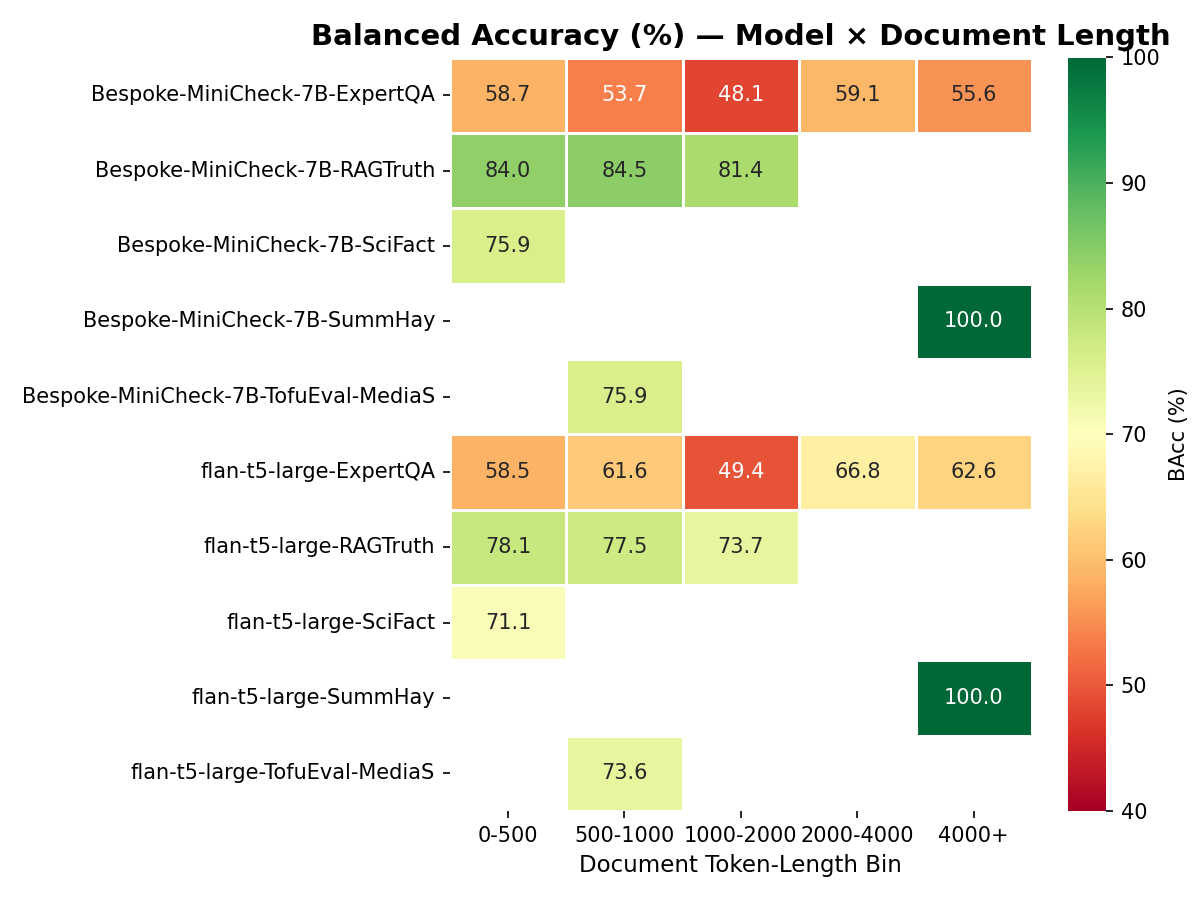
\includegraphics[width=0.8\textwidth]{bacc_heatmap.png}
    \caption{Balanced Accuracy heatmap across models and document length bins.}
    \label{fig:bacc}
\end{figure}

\textbf{2. Extreme Context Capability (SummHay):}
To test extreme scenarios, we evaluated the models on the SummHay dataset, averaging roughly 74,487 tokens per document. Using a sampled setup with cross-topic negative insights, both \texttt{flan-t5-large} and \texttt{Bespoke-MiniCheck-7B} achieved 100\% BAcc, proving that the underlying MiniCheck chunking architecture successfully evaluates massive documents without catastrophic system failure.

\textbf{3. Efficiency and Latency Analysis:}
While BAcc remained relatively stable across the board, computational efficiency took a significant hit on long contexts. As illustrated in Figure~\ref{fig:spm}, inference latency increases dramatically for massive documents. For example, \texttt{flan-t5-large} processed the standard RAGTruth dataset in roughly 796 seconds total, but scaling up to the massive $\sim$74k-token SummHay documents required over 434 seconds for just a 100-sample subset. \texttt{Bespoke-MiniCheck-7B} exhibited even greater latency costs, requiring 1,542 seconds for the SummHay subset.

\begin{figure}[H]
    \centering
    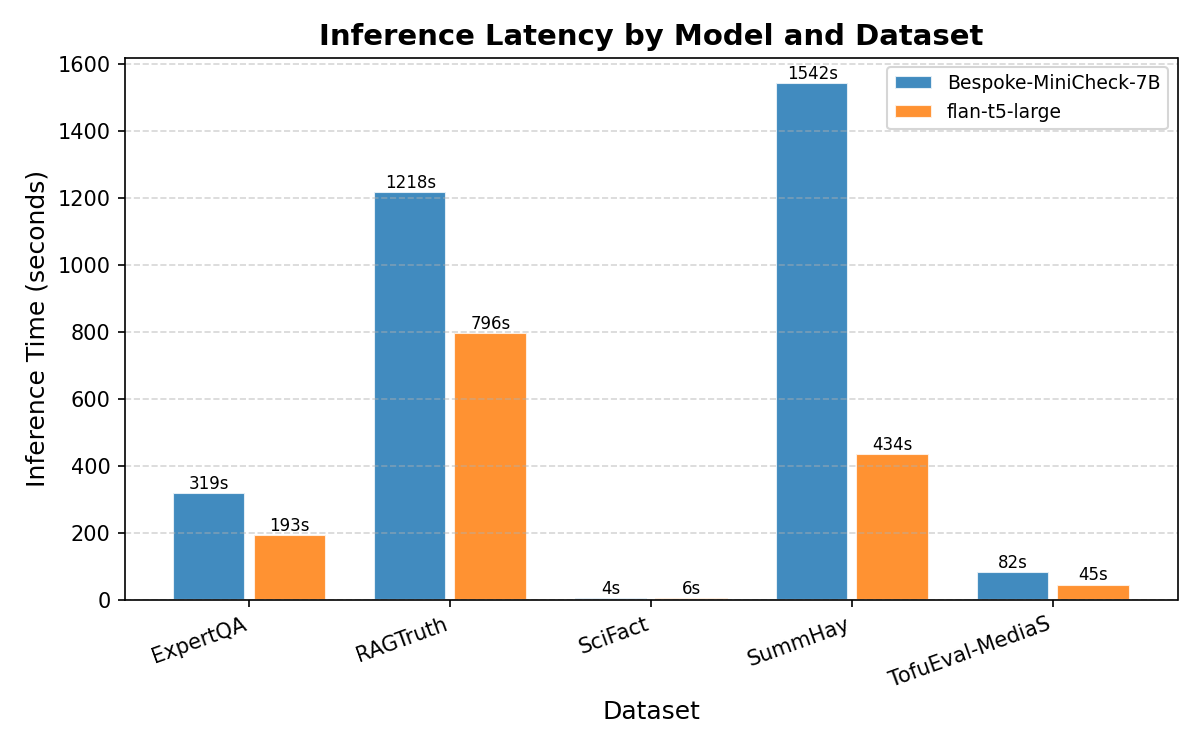
\includegraphics[width=0.8\textwidth]{latency_bar.png}
    \caption{Inference Time (seconds) by Model and Dataset.}
    \label{fig:spm}
\end{figure}

\section*{F. Plan for Completion}

\textbf{Remaining Timeline (Milestones):}
\begin{itemize}[leftmargin=*]
    \item \textbf{Week 5-6: Extended Dataset Evaluation OR Advanced Adversarial Injection:} Depending on feasibility, we will explore one of two paths. We may either expand our evaluation across more pure long-context subsets from the LLM-AggreFact benchmark, or dynamically inject purely adversarial, synthetically generated hallucinatory strings directly into the optimal retrieval chunks to trick the MiniCheck chunking logic.
    \item \textbf{Week 7-8: Final Analysis and API Benchmarks:} As an additional possibility, we may run a subset of our tests against commercial models to benchmark resilience. However, due to constraints (lack of paid GPT-4o API access), this would likely be restricted to free-tier model APIs. The final report will assemble these observations.
\end{itemize}

\bibliographystyle{unsrt}
\bibliography{refs}

\end{document}
